\subsection{Corpus Generieren}
    In früheren Versuchen wurden die unter \texttt{http://dumps.wikimedia.org/backup-index.html} zum download verfügbaren Artikel von der Wikipedia als \emph{Corpus} verwendet. Allerdings war hier schnell zu erkennen, dass das daraus generierte \emph{Sprachmodell} schlecht für einen \emph{Talker} geeignet sind. So dürfte das Wort \texttt{ich} für einen Nutzer ein sehr wichtiges Wort sein. Bei Wikipedia ist das Auftreten dieses Wortes jedoch eher seltener Wort zu vermuten.
    
    Letztendlich wurden drei verschiedene \emph{Corpora} generiert.
    Alle Texte sind dem Project Gutenberg entnommen.
    
    \begin{description}
		\item[Märchen] besteht aus den drei älteren Märchen: \emph{Alice Abenteuer im Wunderland} \parencite{gutenberg:alice}, \emph{Der Mann im Mond} \parencite{gutenberg:mannImMond} und \emph{Peterchens Mondfahrt} \parencite{gutenberg:mondfahrt}. In diesem Corpus werden alte Rechtschreibung und alte Sprache verwendet. Gleichzeitig sind viele Dialoge enthalten.
        
        \item[Prosa] besteht aus einer Briefsammlung von Wilhelm von Humboldt mit dem Titel \emph{Briefe an eine Frendin} \parencite{gutenberg:briefeFreundin}. Diese Briefe sind in altmodischer Sprache verfasst und in Ich-Form geschrieben.
        
        \item[Simple] ist ein manuell generierter \emph{Corpus} hier sind Sätze wie \texttt{ich habe hunger} enthalten. Also Sätze die zur grundlegenden Kommunikation benötigt werden, wie man sie in einem Reiseführer finden könnte.
            
	\end{description}
        
    \subsubsection*{Text bereinigen}
    \label{clean-up-text}
    
        Zum Testen der folgenden Textoperationen wurde Project Gutenberg's Alice's Abenteuer im Wunderland \parencite{gutenberg:alice} als Ausgangstext verwendet.
        
        Bevor ein Text dem Algorithmus übergeben werden kann muss dieser zuerst bereinigt werden. Dies ist zu großen Teilen mit Reguläreren Ausdrücken möglich. Zu Beginn werden die in \autoref{fig:regexpSpecialChars} aufgelisteten Sonderzeichen aus dem Text entfernt.
            
        \begin{figure}[H]
            \centering
            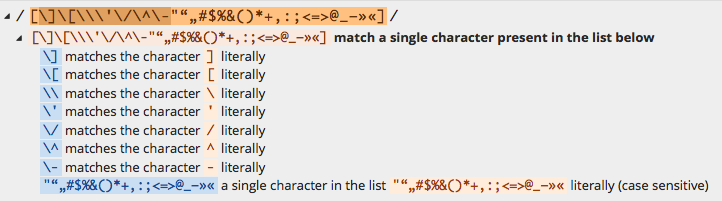
\includegraphics[width=0.8\linewidth]{images/regexpSpecialChars.png}
  			\caption{Regulärer Ausdruck zum finden von Sonderzeichen} \parencite{regex101:specialChars}
			\label{fig:regexpSpecialChars}
		\end{figure}
            
		Auch wenn in deutschem Text Groß- und Kleinschreibung den Unterschied zwischen zwei Worten ausmachen kann, lieferte die Umwandlung des kompletten Textes in Kleinbuchstaben subjektiv bessere Ergebnisse in der Wortvorhersage. Da somit ein Wort am Satzanfang keinen Unterschied zu dem gleichen Wort an einer anderen Position im Satz aufweist. Ein Satzanfang folgt in der Regel auf ein Satzende darum wird im Folgenden von einem \emph{Satzumbruch} gesprochen. Um den \emph{Corpus} weiter zu vereinfachen wurden die in \autoref{tab:wordTags} gelisteten Ersetzungen eingeführt.
        
		\begin{figure}[H]
			\centering
                
			\begin{tabular}{ l | l }
                Ersetzung & Bedeutung \\ \hline \hline
                \texttt{<number>} & Zahlen \\ \hline
                \texttt{<abbrevation>} & bekannte Abkürzungen \\ \hline
                \texttt{<unkown>} & Wörter mit nur einem Buchstaben \\ \hline
                \texttt{<S/>} & \emph{Satzumbruch}
            \end{tabular}
            \caption{ }
			\label{tab:wordTags}
		\end{figure}
            
        Auch \emph{Satzumbrüche} können mit Reguläreren Ausdrücken gefunden werden. Um möglichst wenige falsch als \emph{Satzumbruch} markierte Stellen zu haben wird ein Satzanfang eher konservativ mit dem in \autoref{fig:regexpSentence1} erklärten Regulärem Ausdruck definiert. Ein \emph{Satzumbruch} beginnt also mit einem Kleinbuchstaben vor einem Punkt, einem Fragezeichen oder einem Ausrufezeichen. Darauf folgt ein \emph{white space character} vor einem Großbuchstaben oder einer Ziffer.
            
		\begin{figure}[H]
        	\centering
            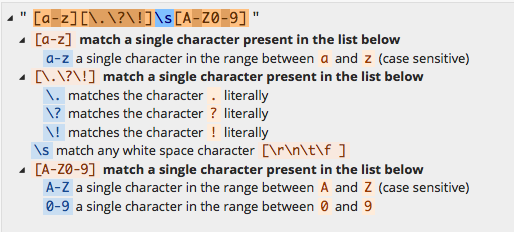
\includegraphics[width=0.8\linewidth]{images/regexpSentence.png}
  			\caption{Regulärer Ausdruck zum finden von \emph{Satzumbrüchen} \parencite{regex101:sentence1}}
			\label{fig:regexpSentence1}
		\end{figure}
        \newpage
            
		Diese Definition übersieht Satzenden am Ende eines Absatzes, darum wird noch ein weiterer in \autoref{fig:regexpSentence2} gezeigter Regulärer Ausdruck verwendet. In kombination konnten mit diesen Beiden Ausdrücken in Tests fast alle \emph{Satzumbrüche} gefunden werden.
            
        \begin{figure}[H]
			\centering
            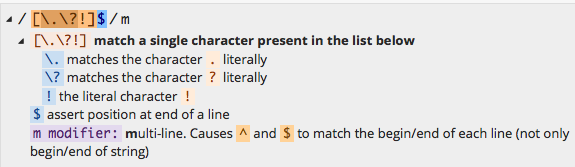
\includegraphics[width=0.8\linewidth]{images/regexpSentence2.png}
  			\caption{zweiter Regulärer Ausdruck zum finden von \emph{Satzumbrüchen} \parencite{regex101:sentence2}}
			\label{fig:regexpSentence2}
		\end{figure}
            
        Dank der Ersetzung von Abkürzungen können Falsche Erkennungen reduziert werden, da Abkürzungen wie \enquote{\texttt{z. B.}} nicht mehr als \emph{Satzumbruch} erkannt werden. Darum wird die Ersetzung von Abkürzungen vor dem Finden von \emph{Satzumbrüchen} vorgenommen. Dies gilt auch für das Entfernen von Sonderzeichen, somit wird Beispielsweise auch im Textausschnitt \enquote{\texttt{[\dots]>>hole sie her.<< Und der Henker lief[\dots]}} der \emph{Satzumbruch} erkannt. In \autoref{fig:regexpSpecialChars} wurden darum auch keine Zeichen entfernt die zur Erkennung von \emph{Satzumbrüchen} benötigt werden. Alle anderen Ersetzungen so wie das Umwandeln in Kleinbuchstaben werden nach dem Markieren von \emph{Satzumbrüchen} vorgenommen.
